\section{Anexo 2: Otros experimentos}\label{Anexo:experimentos}

	Este anexo incluye algunos de los experimentos realizados en este TFG y que no han sido incluidos en el capítulo \ref{cap:test}. Estos experimentos están clasificados siguiendo los criterios definidos en dicho capítulo. Existe algún experimento que cubre un caso intermedio y por lo tanto, no ha podido ser clasificado. Sin embargo, también es interesante para evaluar el funcionamiento del actuador. En la siguiente tabla se muestra una relación de los experimentos que se incluyen en este anexo.

\begin{table}[h]
\centering
\scalebox{0.80}[0.90]{
	\begin{tabular}{| c | c | c | c |}
		\hline
		\textbf{Num Exp} & \textbf{Tipo exp} &\textbf{Experimento}  & \textbf{Parámetros PID}\\
		\hline 
			\textbf{5} & 1 &Subida de 19{$^\circ$}C a 24{$^\circ$}C  & $K_{p}=28$ $K_{i}=0,037$  $ K_{d}=300$\\
		\hline
			\textbf{6} & 1 &Subida de 19.5{$^\circ$}C a 23{$^\circ$}C  & $K_{p}=28$ $K_{i}=0,037$  $ K_{d}=300$ \\
		\hline
			\textbf{7} & 1 y 2 & Subida de 19.5{$^\circ$}C a 22{$^\circ$}C & $K_{p}=28$ $K_{i}=0,037$  $ K_{d}=300$\\
				       &          & y bajada de 22{$^\circ$}C a 18{$^\circ$}C & \\
		\hline
			\textbf{8} &  &  Subida de 21{$^\circ$}C a 23{$^\circ$}C  & $K_{p}=28$ $K_{i}=0,037$  $ K_{d}=300$\\
				       &  & y bajada de 23{$^\circ$}C a 21{$^\circ$}C & \\
		\hline	
			\textbf{9} & 3 & Subida de 19{$^\circ$}C a 23,5{$^\circ$}C en pasos de  0,5{$^\circ$}C & $K_{p}=28$ $K_{i}=0,037$  $ K_{d}=300$\\
		\hline
			\textbf{10} & 3 & Subida de 21.5{$^\circ$}C a 23,5{$^\circ$}C en pasos de  0,5{$^\circ$}C  & $K_{p}=28$ $K_{i}=0,037$  $ K_{d}=300$ \\
		\hline
			\textbf{11} & 1 y 4 &  Subida de 19.5{$^\circ$}C a 23{$^\circ$}C & $K_{p}=28$ $K_{i}=0,037$  $ K_{d}=300$\\
				         &          &  y bajada de 23{$^\circ$}C a 21,5{$^\circ$}C en pasos de 0,5{$^\circ$}C & \\
		\hline
			\textbf{12} & 3 & Subida de 19.5{$^\circ$}C a 21{$^\circ$}C en pasos de 0.5{$^\circ$}C& $K_{p}=28$ $K_{i}=0,037$  $ K_{d}=300$\\
		\hline	
\end{tabular}}
\label{tablaA2_1:pruebas}\caption{Características de los experimentos realizados}
 \end{table}

	En cada gráfica aparece la temperatura de la sala (azul), la temperatura óptima (rojo) y el setpoint (verde). No se ha incluido en ninguna gráfica la señal de control debido a que en ocasiones toma valores muy grandes o muy pequeños que impiden ver con claridad el resto de señales. A continuación se muestran las gráficas de los experimentos de la tabla \ref{tablaA2_1:pruebas}.

\newpage

\begin{figure}[H]
\centering
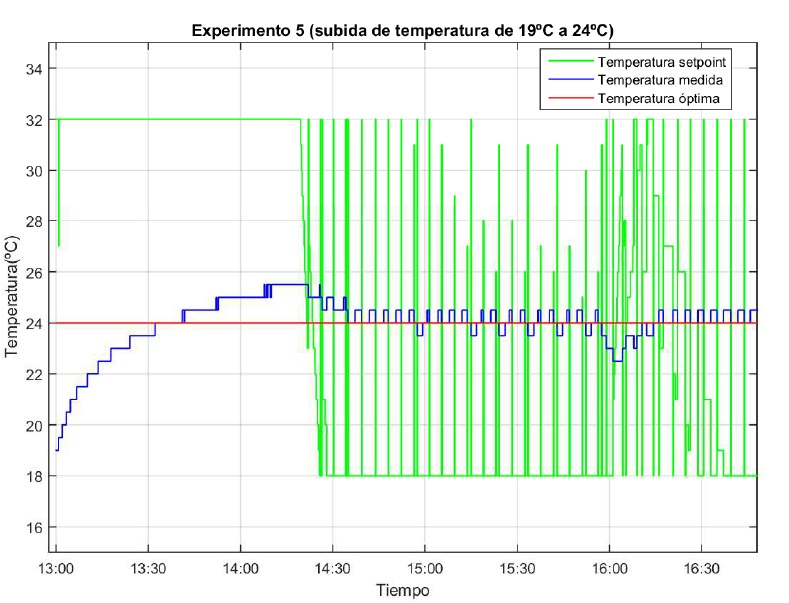
\includegraphics[width=130mm,height=95mm]{imagenes/anexo2/experimento5}
\caption {Gráfica con los resultados del experimento 5}
\label{figA2_1:experimento5}
\end{figure}

\begin{figure}[H]
\centering
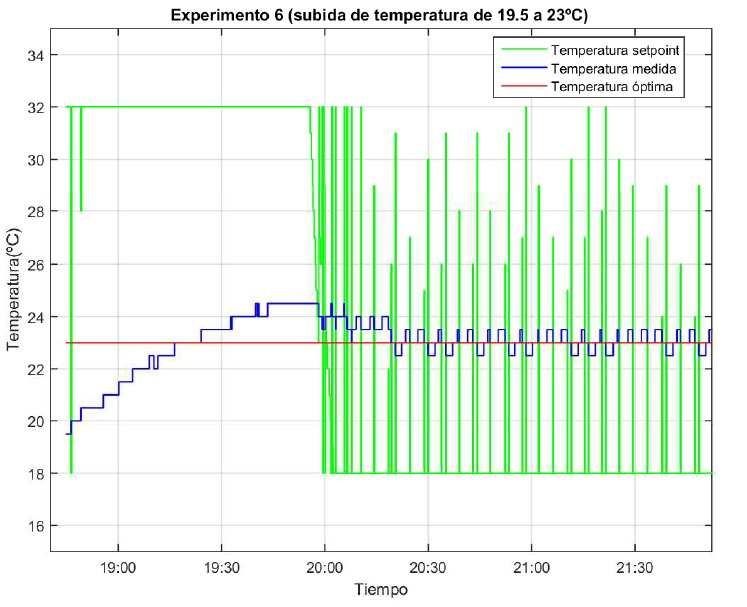
\includegraphics[width=130mm,height=95mm]{imagenes/anexo2/experimento6}
\caption {Gráfica con los resultados del experimento 6}
\label{figA2_2:experimento6}
\end{figure}

\begin{figure}[H]
\centering
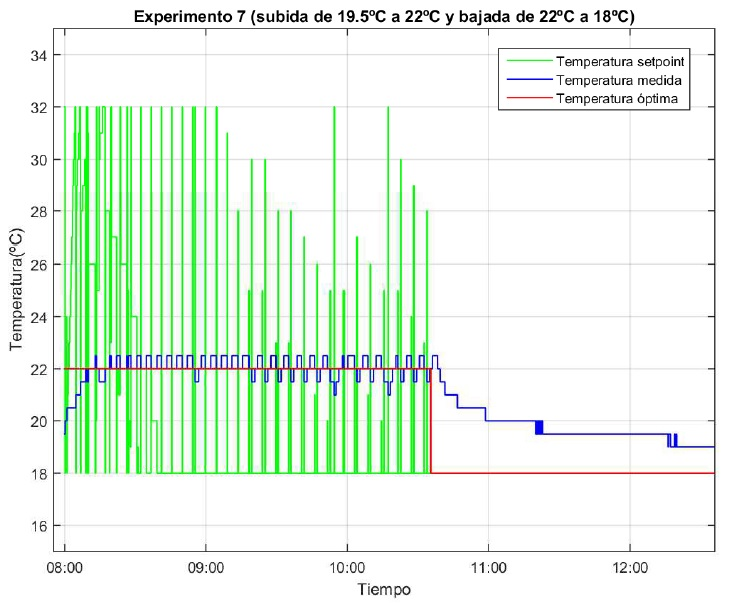
\includegraphics[width=130mm,height=95mm]{imagenes/anexo2/experimento7}
\caption {Gráfica con los resultados del experimento 7}
\label{figA2_3:experimento7}
\end{figure}

\begin{figure}[H]
\centering
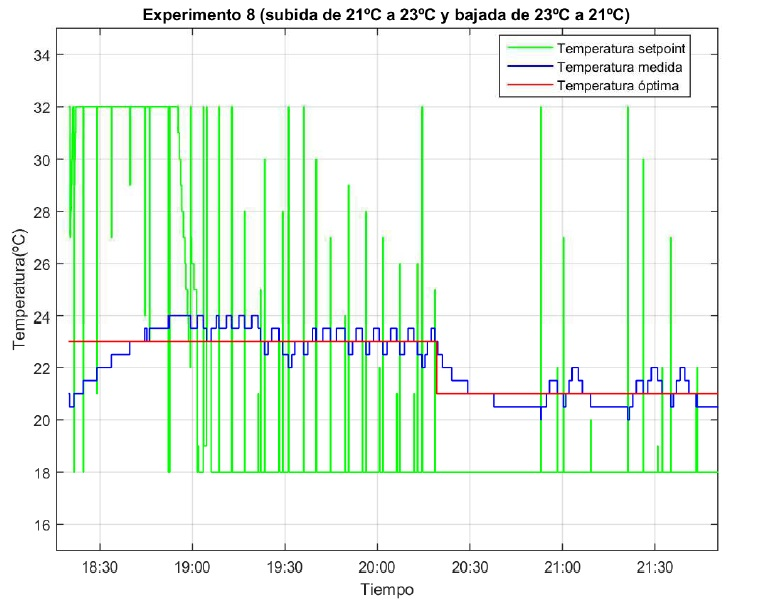
\includegraphics[width=130mm,height=95mm]{imagenes/anexo2/experimento8}
\caption {Gráfica con los resultados del experimento 8}
\label{figA2_4:experimento8}
\end{figure}

\begin{figure}[H]
\centering
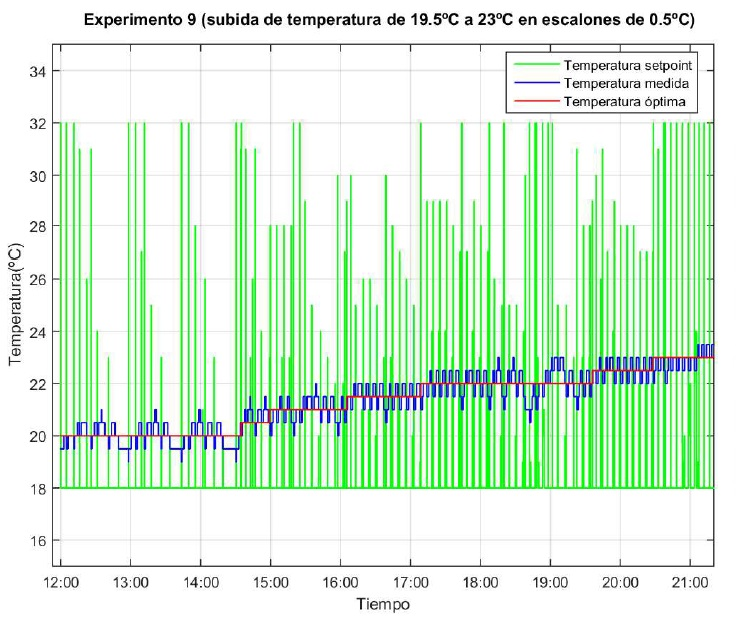
\includegraphics[width=130mm,height=95mm]{imagenes/anexo2/experimento9}
\caption {Gráfica con los resultados del experimento 9}
\label{figA2_5:experimento9}
\end{figure}

\begin{figure}[H]
\centering
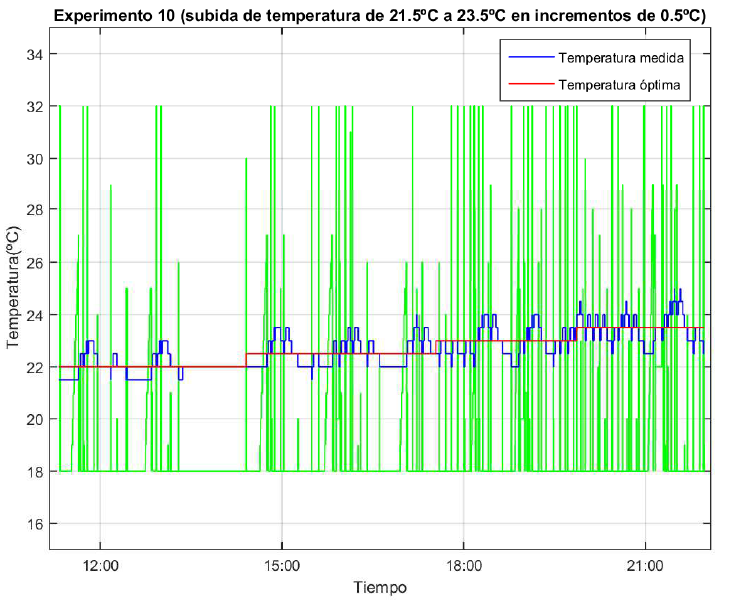
\includegraphics[width=130mm,height=95mm]{imagenes/anexo2/experimento10}
\caption {Gráfica con los resultados del experimento 10}
\label{figA2_6:experimento10}
\end{figure}

\begin{figure}[H]
\centering
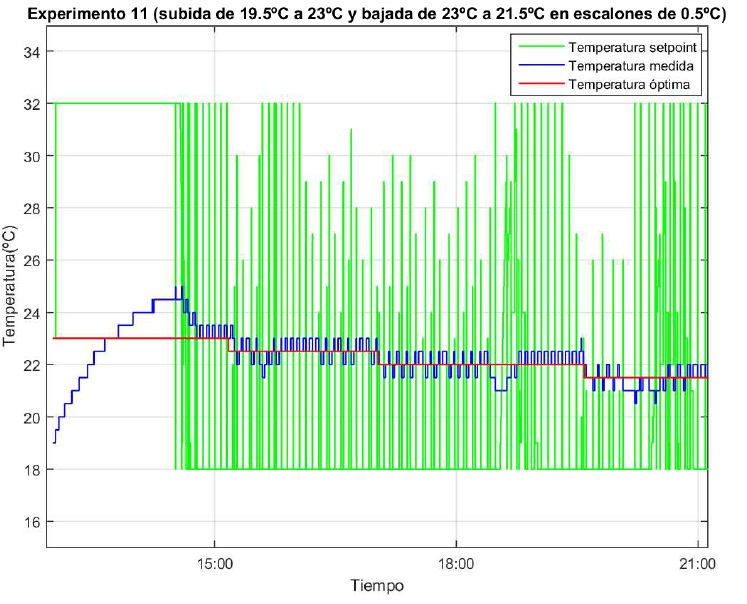
\includegraphics[width=130mm,height=95mm]{imagenes/anexo2/experimento11}
\caption {Gráfica con los resultados del experimento 11}
\label{figA2_7:experimento11}
\end{figure}

\begin{figure}[H]
\centering
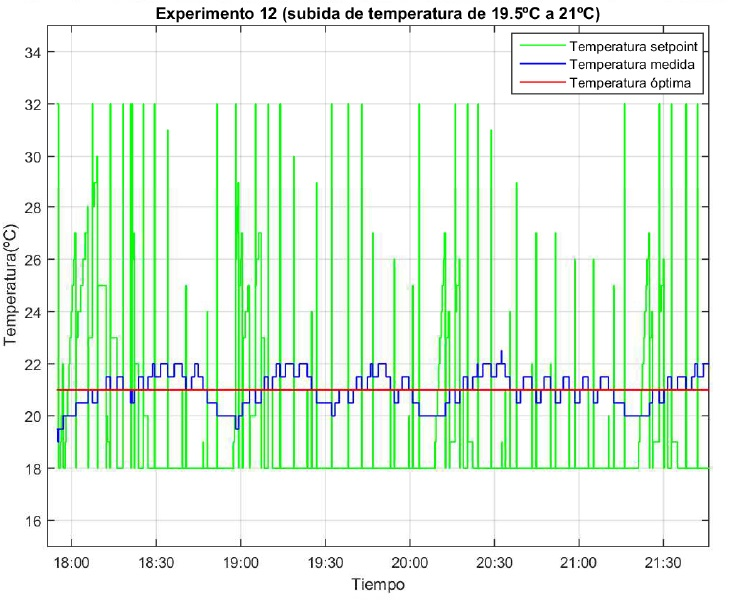
\includegraphics[width=130mm,height=95mm]{imagenes/anexo2/experimento12}
\caption {Gráfica con los resultados del experimento 12}
\label{figA2_8:experimento12}
\end{figure}
